\documentclass[11pt]{article}
\usepackage{projeto-ed}
\usepackage{tikz}

\begin{document}
\ProjetoHeader{Projeto: Fase 1}{Proposta e modelagem}

\InfoBox{\textbf{Objetivo da fase.} Transformar a ideia do jogo em uma primeira especificação computacional. Esta fase vale \textbf{20\% da nota do trabalho prático}. A escolha das estruturas poderá ser revista após o estudo de novos conteúdos.}

\vspace{1cm}
\Campo{Nome provisório do jogo: Blackjack: Jogador vs Computador (DS-Blackjack)}
\Campo{Link da entrega/repositório: https://github.com/ellismorenna/Blackjack.git}


\vspace{1cm}
\section{Equipe e responsabilidades}
\TabelaEquipeCompleta

\section{Proposta do jogo}
\subsection{Ideia e objetivo}
\textit{Descreva o jogo em um parágrafo: contexto, objetivo do jogador e condição geral de sucesso.}\\

 \textit{O jogador deve tentar atingir a maior pontuação possível sem ultrapassar 21. A cada rodada, o jogador pode comprar uma nova carta ou parar. O computador também recebe cartas e segue uma estratégia simples. Ao final, vence quem estiver mais próximo de 21, sem ultrapassá-lo, ou com exatamente 21.}
\AnswerSpace{5mm}

\subsection{Regras essenciais}
\textit{Liste apenas as regras necessárias para compreender uma partida, incluindo início, ações permitidas, progressão e término.} \\

\begin{enumerate}
    \item \textit{}{Distribuição Inicial:} No início de cada partida, um baralho de 52 cartas é embaralhado e são distribuídas duas cartas ao jogador e duas ao computador (uma aberta e uma oculta).
    \item \textit{Valores:} Cartas de 2 a 10 mantem seu valor nominal; J, Q, K valem 10; o Ás vale 11 ou 1 (ajustado automaticamente).
    \item \textit{Turno do Jogador:} O jogador pode escolher entre comprar uma carta ou parar. Se ultrapassar 21 ele estoura e perde.
    \item \textit{Turno do Computador:} Ao escolher, o computador revela a carta oculta e compra cartas automaticamente enquanto sua soma for menor que 17.
    \item \textit{Vitória:} Vence quem estiver mais próximo de 21 sem estourar.
    
\end{enumerate}
\AnswerSpace{5mm}

\vspace{2mm}
\section{Modelagem inicial}
\subsection{Entidades e informações armazenadas}
\begin{tabularx}{\textwidth}{X X X}
  \toprule
  Entidade & Dados necessários & Papel no jogo \\
  \midrule
   Carta & naipe, valor e pontuação & Representa cada carta disponível no baralho e utilizada nas mãos\\
   \\
   Baralho & Conjunto e quantidade de cartas disponíveis & Armazena as cartas que podem ser compradas durante a partida \\
   \\
   Mão & cartas que pertencem ao jogador/computador e pontuação atual & Cartas na mão de cada participante \\
   \\
   Partida & mão do jogador, mão do computador, estado da partida e resultado & Controla o andamento da partida e determina seu resultado\\
   \\
  \bottomrule
\end{tabularx}

\subsection{TADs propostos}
\begin{tabularx}{\textwidth}{p{3cm} X X}
  \toprule
  TAD & Responsabilidade & Operações previstas \\
  \midrule
   Baralho & Gerenciar as cartas disponíveis para serem retiradas durante a partida. & criarBaralho(), embaralhar(), retirarCarta(), verificarVazio(),  liberarBaralho() \\
   \\
   Mão & Gerenciar as cartas pertencentes aos jogadores (pessoa e computador) e calcular sua pontuação & criarMao(), adicionarCarta(), calcularPontuacao(), limparMao(), liberarMao() \\
   \\
  \bottomrule
\end{tabularx}

\subsection{Estruturas de dados candidatas}
\textit{Indique pilha, fila, lista ou outra estrutura considerada. Relacione suas propriedades às operações e regras do jogo. Se houver alternativas, registre a dúvida que será investigada.}
\\
\\
\textit{Baralho - Pilha: O baralho sera representado por uma pilha, porque, a partir do topo da estrutura, as cartas serão retiradas uma por vez. Será utilizada operações da pilha para retirar uma carta durante a partida e construir o baralho no começo da partida}
\\
\\
\textit{Mão - Lista encadeada: uma lista encadeada representará a mão de cada participante. A cada compra, uma nova carta sera adicionada à lista, demonstrando dinamicamente a mão de cada um dos jogadores.}
\\
\\
\textit{Inicialmente essas serão as estruturas utilizadas, entretando a implementação será devidamente avaliada durante a Fase 2 para verificar se essas estruturas atendem adequadamente às operações necessárias. }
\AnswerSpace{5mm}

\subsection{Esquema da solução}
\textit{Insira um diagrama simples relacionando entidades, TADs, módulos e fluxo principal do jogo. O diagrama pode ser substituído por uma figura exportada.}
\begin{center}
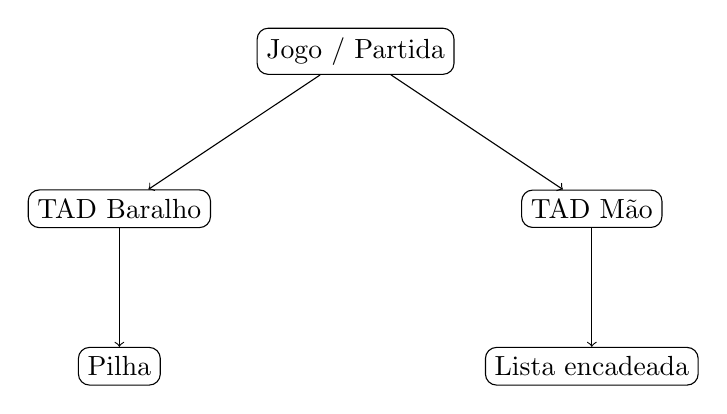
\begin{tikzpicture}

    \node[draw, rounded corners] (jogo) at (0,4)
        {Jogo / Partida};

    \node[draw, rounded corners] (baralho) at (-3,2)
        {TAD Baralho};

    \node[draw, rounded corners] (mao) at (3,2)
        {TAD Mão};

    \node[draw, rounded corners] (pilha) at (-3,0)
        {Pilha};

    \node[draw, rounded corners] (lista) at (3,0)
        {Lista encadeada};

    \draw[->] (jogo) -- (baralho);
    \draw[->] (jogo) -- (mao);

    \draw[->] (baralho) -- (pilha);
    \draw[->] (mao) -- (lista);

\end{tikzpicture}
\end{center}
\\

\begin{center}
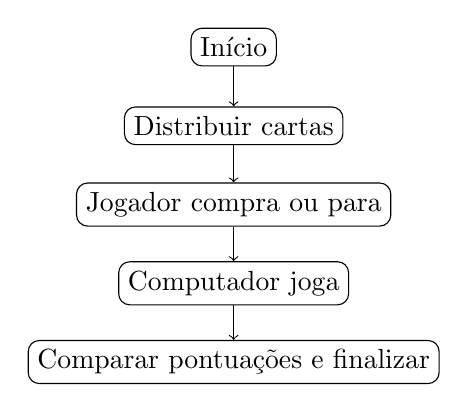
\begin{tikzpicture}

\node[draw, rounded corners] (inicio) at (0,0) {Início};
\node[draw, rounded corners] (cartas) at (0,-1) {Distribuir cartas};
\node[draw, rounded corners] (jogador) at (0,-2) {Jogador compra ou para};
\node[draw, rounded corners] (computador) at (0,-3) {Computador joga};
\node[draw, rounded corners] (resultado) at (0,-4) {Comparar pontuações e finalizar};

\draw[->] (inicio) -- (cartas);
\draw[->] (cartas) -- (jogador);
\draw[->] (jogador) -- (computador);
\draw[->] (computador) -- (resultado);

\end{tikzpicture}
\end{center}

\section{Organização preliminar do programa}
\begin{tabularx}{\textwidth}{p{4cm} X X}
  \toprule
  Módulo/arquivo & Responsabilidade & Dependências principais \\
  \midrule
   main.c & Iniciação do programa e controle do ciclo principal & jogo.h, inteface.h\\
   \\
   jogo.c / jogo.h & Controlar as regras e o estado da partida & baralho.h, mao.h, carta.h\\
   \\
   baralho.c / baralho.h & criar, embaralhar e retirar cartas do baralho & carta.h, pilha.h \\
   \\
   mao.c / mao.h & Armazenar as cartas de cada jogador e calcular pontuação & carta.h, lista.h\\
   \\
   cartas.c / cartas.h & Representar e manipular uma carta & \\
   \\
   pilhas.c / pilha.h & Implementar as operações de pilha & \\
   \\
   lista.c / lista.h & Implementar as operações da lista encadeada &  \\
   
   interface.c / interface.h & Mostrar o jogo e receber ações do jogador. & jogo.h\\
   
   
  \bottomrule
\end{tabularx}

\section{Plano para a Fase 2}
\begin{tabularx}{\textwidth}{X p{4cm} p{4cm}}
  \toprule
  Tarefa & Responsável(is) & Evidência de conclusão \\
  \midrule
   Implementar e integrar os TADs, estruturas de dados, regras da partida e interface gráfica, realizando os testes necessários & Ellis Morenna & Versão intermediária executável, com as principais operações dos TADs, fluxo básico da partida e interface gráfica funcionando\\
   
  \bottomrule
\end{tabularx}

\vspace{1cm}
\DeclaracaoIA

\section{Checklist da entrega}
\begin{EntregaChecklist}
  \item ideia e regras resumidas;
  \item entidades e informações armazenadas;
  \item TADs e operações preliminares;
  \item estruturas candidatas e justificativa inicial;
  \item organização dos módulos e divisão do trabalho;
  \item diagrama da modelagem;
  \item declaração de IA preenchida.
\end{EntregaChecklist}



\end{document}
